\documentclass{article}
\usepackage{graphicx} % Required for inserting images
\usepackage{tikz}
\usetikzlibrary{arrows,automata,positioning,matrix}
\usepackage[pdftex]{pict2e}
\title{tikz}
\author{ashish.thapa477 }
\date{May 2023}

\begin{document}

\maketitle

\section{Introduction}


\begin{figure}[h]
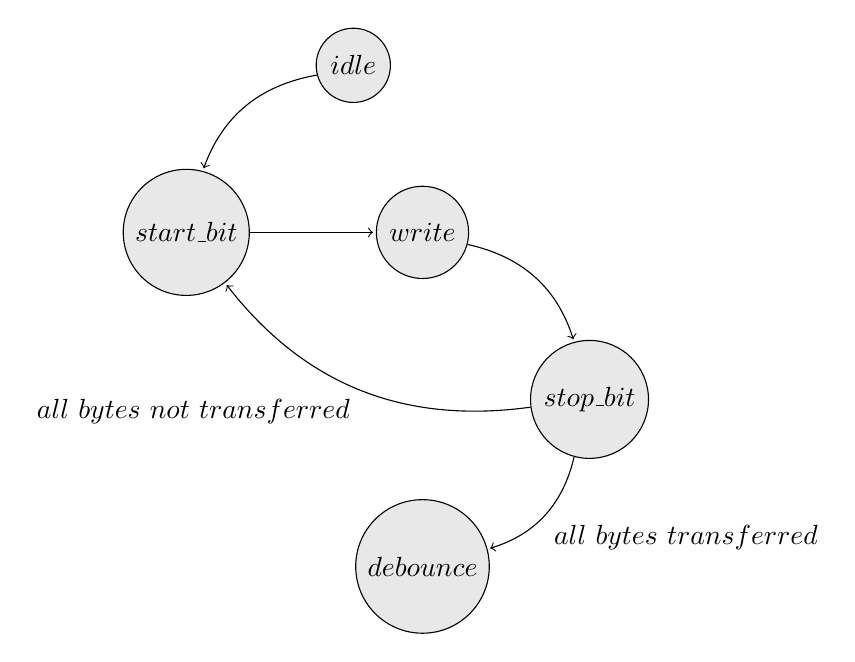
\begin{tikzpicture}[shorten >=1pt,node distance=3cm,auto]
  \tikzstyle{every state}=[fill={rgb:black,1;white,10}]

  \node[state]   (idle)                      {$idle$};
  \node[state] (startbit) [below left of=idle]  {$start\_bit$};
  \node[state]           (write) [right of=startbit]     {$write$};
  \node[state] (stop) [below right of=write] {$stop\_bit$};
  \node[state]           (debounce) [below left of=stop]     {$debounce$};

\path[->]
(idle) edge [bend right] node {} (startbit)
(startbit) edge node {} (write)
(write) edge [bend left] node {} (stop)
(stop) edge [bend left] node {$all\ bytes\ not\ transferred$} (startbit)
(stop) edge [bend left] node {$all\  bytes\ transferred$} (debounce);
\end{tikzpicture}
\caption{State diagram for UART Protocol} 
\end{figure}

\begin{figure}[h]
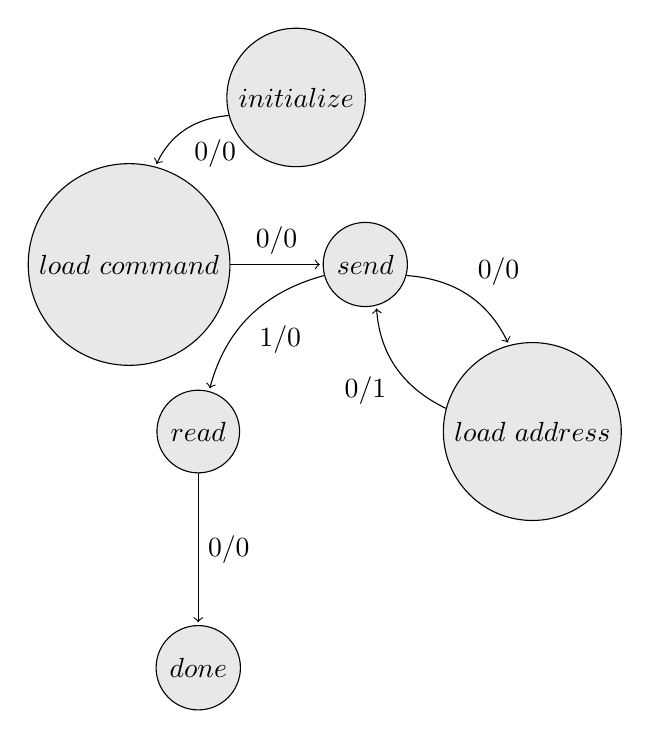
\begin{tikzpicture}[shorten >=1pt,node distance=3cm,auto]
  \tikzstyle{every state}=[fill={rgb:black,1;white,10}]

  \node[state]   (init)                      {$initialize$};
  \node[state] (loadcmd) [below left of=init]  {$load\ command$};
  \node[state]           (send) [right of=loadcmd]     {$send$};
  \node[state] (loadaddr) [below right of=send] {$load\ address$};
  \node[state]           (read) [below left of=send]     {$read$};
  \node[state]           (done) [below of=read]     {$done$};

\path[->]
(init) edge [bend right] node {$0/0$} (loadcmd)
(loadcmd) edge node {$0/0$} (send)
(send) edge [bend left] node {$0/0$} (loadaddr)
(loadaddr) edge [bend left] node {$0/1$} (send)
(send) edge [bend right] node {$1/0$} (read)
(read) edge node {$0/0$} (done);
\end{tikzpicture}
\caption{State diagram for SPI Flash Protocol}
\end{figure}

% CPU
\begin{figure}[h]
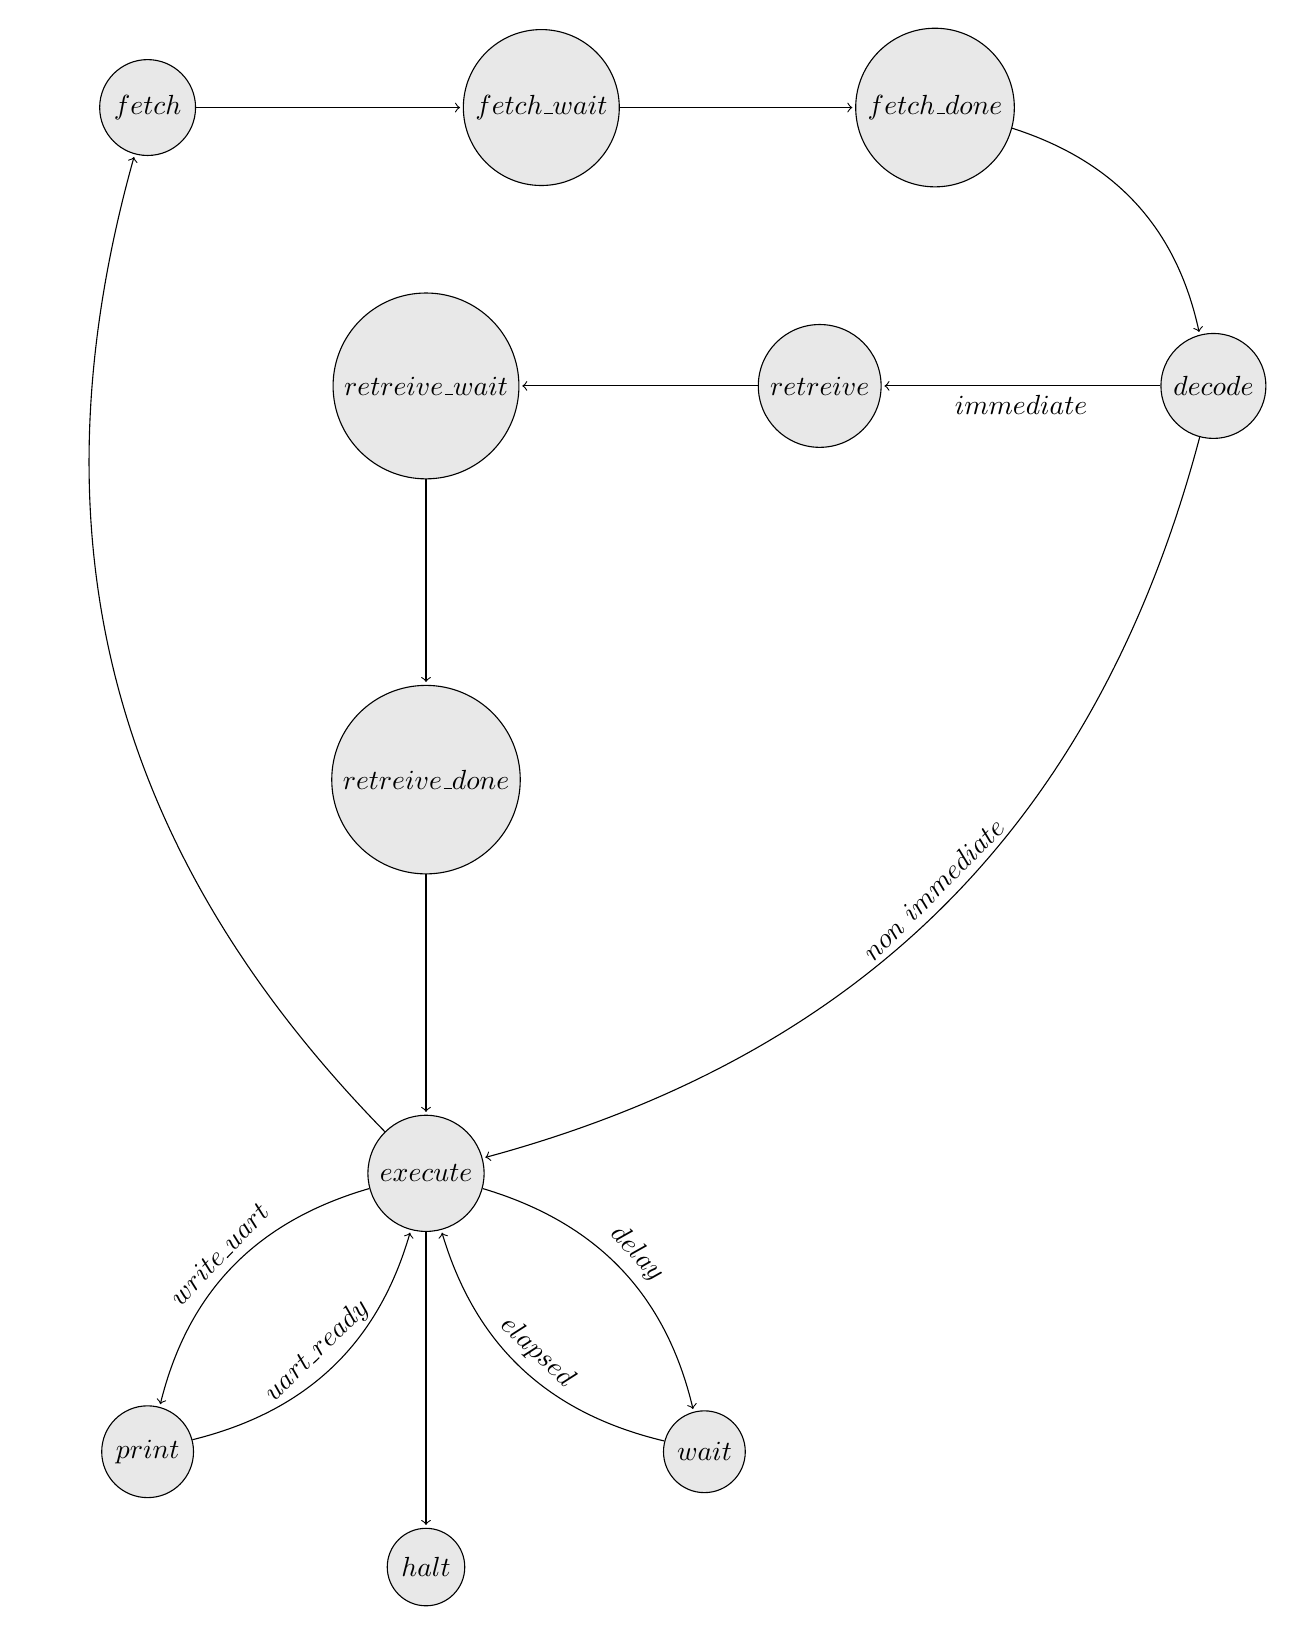
\begin{tikzpicture}[shorten >=1pt,node distance=5cm,auto]
  \tikzstyle{every state}=[fill={rgb:black,1;white,10}]

  \node[state]   (fetch)                      {$fetch$};
  \node[state] (fwait) [right of=fetch]  {$fetch\_wait$};
  \node[state]           (fdone) [right of=fwait]     {$fetch\_done$};
  \node[state] (decode) [below right of=fdone] {$decode$};
  \node[state]           (retreive) [left of=decode]     {$retreive$};
  \node[state]           (rwait) [left of=retreive]     {$retreive\_wait$};
  \node[state]           (rdone) [below of=rwait]     {$retreive\_done$};
  \node[state]           (execute) [below of=rdone]     {$execute$};
  \node[state]           (print) [below left of=execute]     {$print$};
  \node[state]           (wait) [below right of=execute]     {$wait$};
  \node[state]           (halt) [below of=execute]     {$halt$};
\path[->]
(fetch) edge  node {} (fwait)
(fwait) edge  node {} (fdone)
(fdone)  edge [bend left]  node {} (decode)
(decode) edge  node {$immediate$}  (retreive)
(decode) edge [bend left] node [sloped] {$non\ immediate$} (execute)
(retreive) edge node {} (rwait)
(rwait) edge  node {} (rdone)
(rdone) edge  node {} (execute)
(execute) edge [bend right]  node [sloped] {$write\_uart$} (print)
(execute) edge [bend left]  node [sloped] {$delay$} (wait)
(print) edge [bend right]  node [sloped] {$uart\_ready$} (execute)
(wait) edge [bend left]  node[sloped] {$elapsed$} (execute)
(execute) edge node {} (halt)
(execute) edge [bend left] node {} (fetch);
\end{tikzpicture}
\caption{State diagram for CPU}
\end{figure}

\begin{figure}
\setlength{\unitlength}{0.8cm}
\begin{picture}(16,1)
  \multiput(0,0)(0,1){2}{\line(1,0){16}}
  \multiput(0,0)(1,0){17}{\line(0,1){1}}
  \put(0,-1){\line(1,0){1}}
  \put(0,-1){\line(0,1){1}}
  \put(0.1,-0.7){$CM$}
  \put(1,-1){\line(0,1){1}}
  
  \put(1,-1){\line(1,0){5}}
  \put(1,-1){\line(0,1){1}}
  \put(1.2,-0.7){$COMMANDS$}
  \put(6,-1){\line(0,1){1}}
  
  \put(6,-1){\line(1,0){10}}
  \put(6,-1){\line(0,1){1}}
  \put(6.2,-0.7){$VARIATION$}
  \put(16,-1){\line(0,1){1}}
\end{picture}
\vspace{0.4cm}
\caption{ISA}
\end{figure}


\end{document}
